\section{FCNC and rare decays}

\begin{figure}
    \centering
    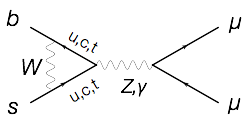
\includegraphics[width=0.45\textwidth]{fig/RareBs2MuMu}
    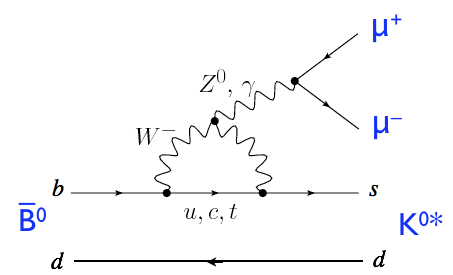
\includegraphics[width=0.45\textwidth]{fig/RareKstarMuMu}
    \caption{Important rare decays being studied at LHCb and elsewhere: \prt{B_s \to \mu^+ \mu^-} and \prt{\Bdo \to K^{*0} \mu^+ \mu^-}\label{fig:RareDecays}}
\end{figure}
CP violation measurements are not the only type of measurement that is sensitive to new physics in Flavour Changing Neutral Currents. There is a host of "rare decays" that is being studied. Particularly important in this context are \prt{\Bdo \to \mu^+ \mu^-}, \prt{B_s \to \mu^+ \mu^-} and \prt{\Bdo \to K^{*0} \mu^+ \mu^-}. The relevant Feynman diagrams are shown in \figref{fig:RareDecays}. Especially in \prt{\Bdo \to K^{*0} \mu^+ \mu^-}, and in other "electroweak penguin" diagrams, there have been some very intriguing hints of deviations from the Standard Model. Note that $\Bdo, \Bso \to \mu^+ \mu^-$ is not only suppressed because of FCNC, but also helicity-suppressed (one of the muons is forced to have the "wrong" helicity). The discovery of $\Bso \to \mu^+ \mu^-$ was a remarkable combined achievement by LHCb \&\ CMS, who measured a branching fraction for $\Bso \to \mu^+ \mu^-$ of $2.8^{+0.7}_{-0.6} \cdot 10^{-9}$ (about in line with SM expectations).


